This chapter discusses the security solution implementation for the development CheFeed.  It will discuss what security implementation has been put in place for the API and client-side development, with the help of programming libraries.

\section{API Implementation}
The API for CheFeed is implemented with FastAPI. A python library to develop APIs with Python 3.6 and above with support for standard Python type hints. FastAPI is chosen for the API implementation due to it being fast and having built-in security features such as authentication. Furthermore, FastAPI also has several external plugins available to enhance and speed up development time. Table \ref{tab:implemented-security-controls} describes the implemented security controls for the API.

\begin{table}
    \centering
    \caption{Implemented security controls}
    \label{tab:implemented-security-controls}
    \begin{tabulary}{1.0\textwidth}{|l|L|l|}
        \hline
        \textbf{ID} & \textbf{Security control} & \textbf{Done} \\
        \hline
        \textbf{4.1} & If the app provides users access to a remote service, some form of authentication, such as username/password authentication, is performed at the remote endpoint & Yes \\
        \hline
        \textbf{4.3} & If stateless token-based authentication is used, the server provides a token that has been signed using a secure algorithm & Yes \\
        \hline
        \textbf{4.4} & The remote endpoint terminates the existing session when the user logs out & Yes \\
        \hline
        \textbf{4.5} & A password policy exists and is enforced at the remote endpoint & Yes \\
        \hline
        \textbf{4.7} & Sessions are invalidated at the remote endpoint after a predefined period of inactivity and access tokens expire & Yes \\
        \textbf{4.12} & Authorization models should be defined and enforced at the remote endpoint & Yes \\
        \hline
    \end{tabulary}
\end{table}

\subsection{Authentication and Session Management}
FastAPI on its own can be used to develop authentication mechanisms. However, the process can be time consuming. Therefore, an external plugin was added to the source code. The plugin \emph{fastapi-users} provides all the features needed to quickly develop user registration, authentication, and options to manage user sessions. Furthermore, it supports both SQL databases and MongoDB. 

\subsubsection{Authentication Backend}
Fastapi-users provides methods to manage tokens. The first part is called the \emph{transport} which is responsible for managing how the token is being carried over the request. The second part is called the \emph{transport}, and it is responsible for managing how the token is generated and secured. A combination of the transport and strategy is called the \emph{authentication backend} by fastapi-users.

For CheFeed, a \emph{bearer} token transport is implemented together with a separate database to store the token. As seen previously in figure \ref{fig:sys-arch} the token is stored in a Redis database. Therefore, user authentication is stateless and token-based. The implementation of the authentication backend using fastapi-users as seen in figure \ref{code:api-auth-backend}, ensures that the security controls \emph{4.3}, \emph{4.4} and \emph{4.12} from table \ref{tab:auth-and-session-summary-requirements} are in implemented. 

\paragraph{Appropriate Authentication}
Fastapi-users includes authentication routes to handle user login and user logout without any customization needed. However, the authentication backend and login manager need to be implemented as seen in figure \ref{code:api-auth-backend} and figure \ref{code:api-login-manager}. With those implemented, the authentication route can be implemented as seen in figure \ref{code:api-router}.

\begin{figure}
    \centering
    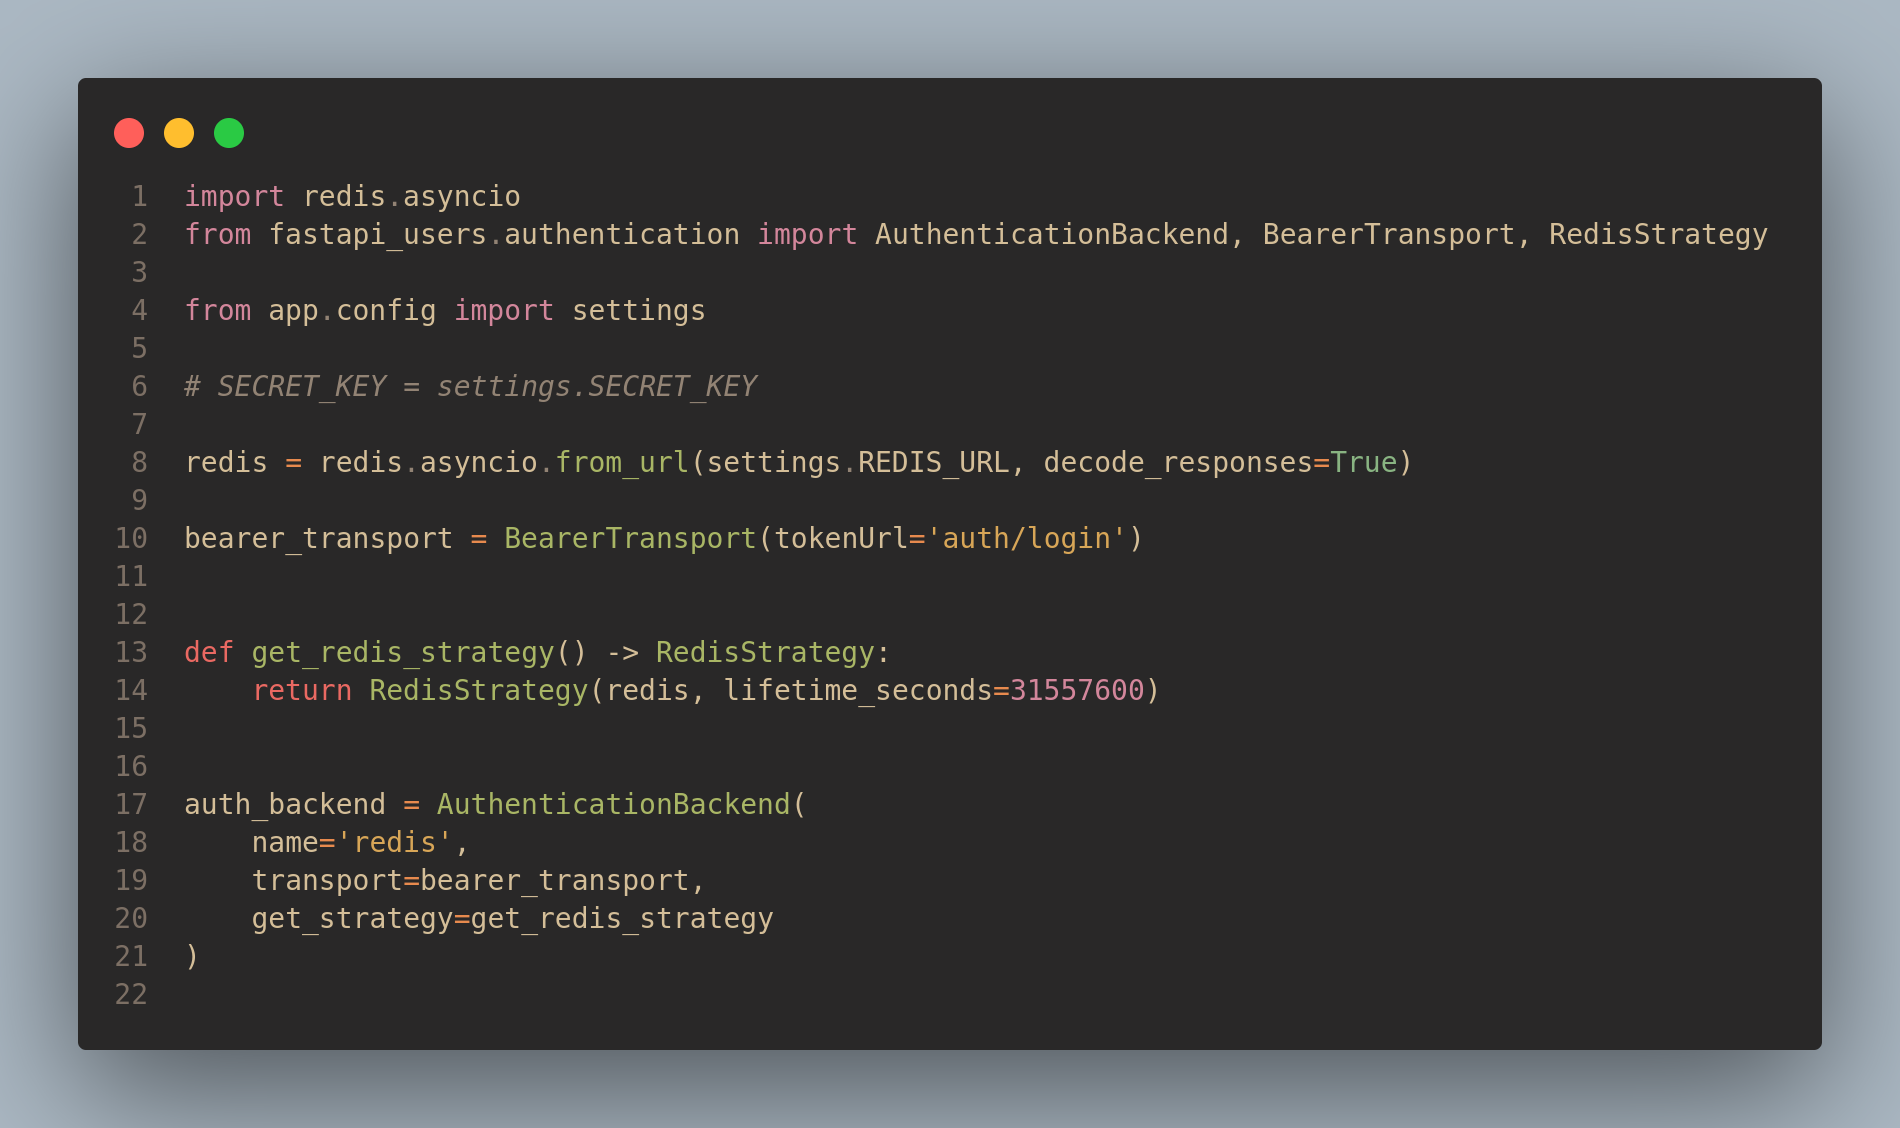
\includegraphics[width=\textwidth]{chapter-5/api-auth-backend}
    \caption{API authentication backend with fastapi-users}
    \label{code:api-auth-backend}
\end{figure}

\begin{figure}
    \centering
    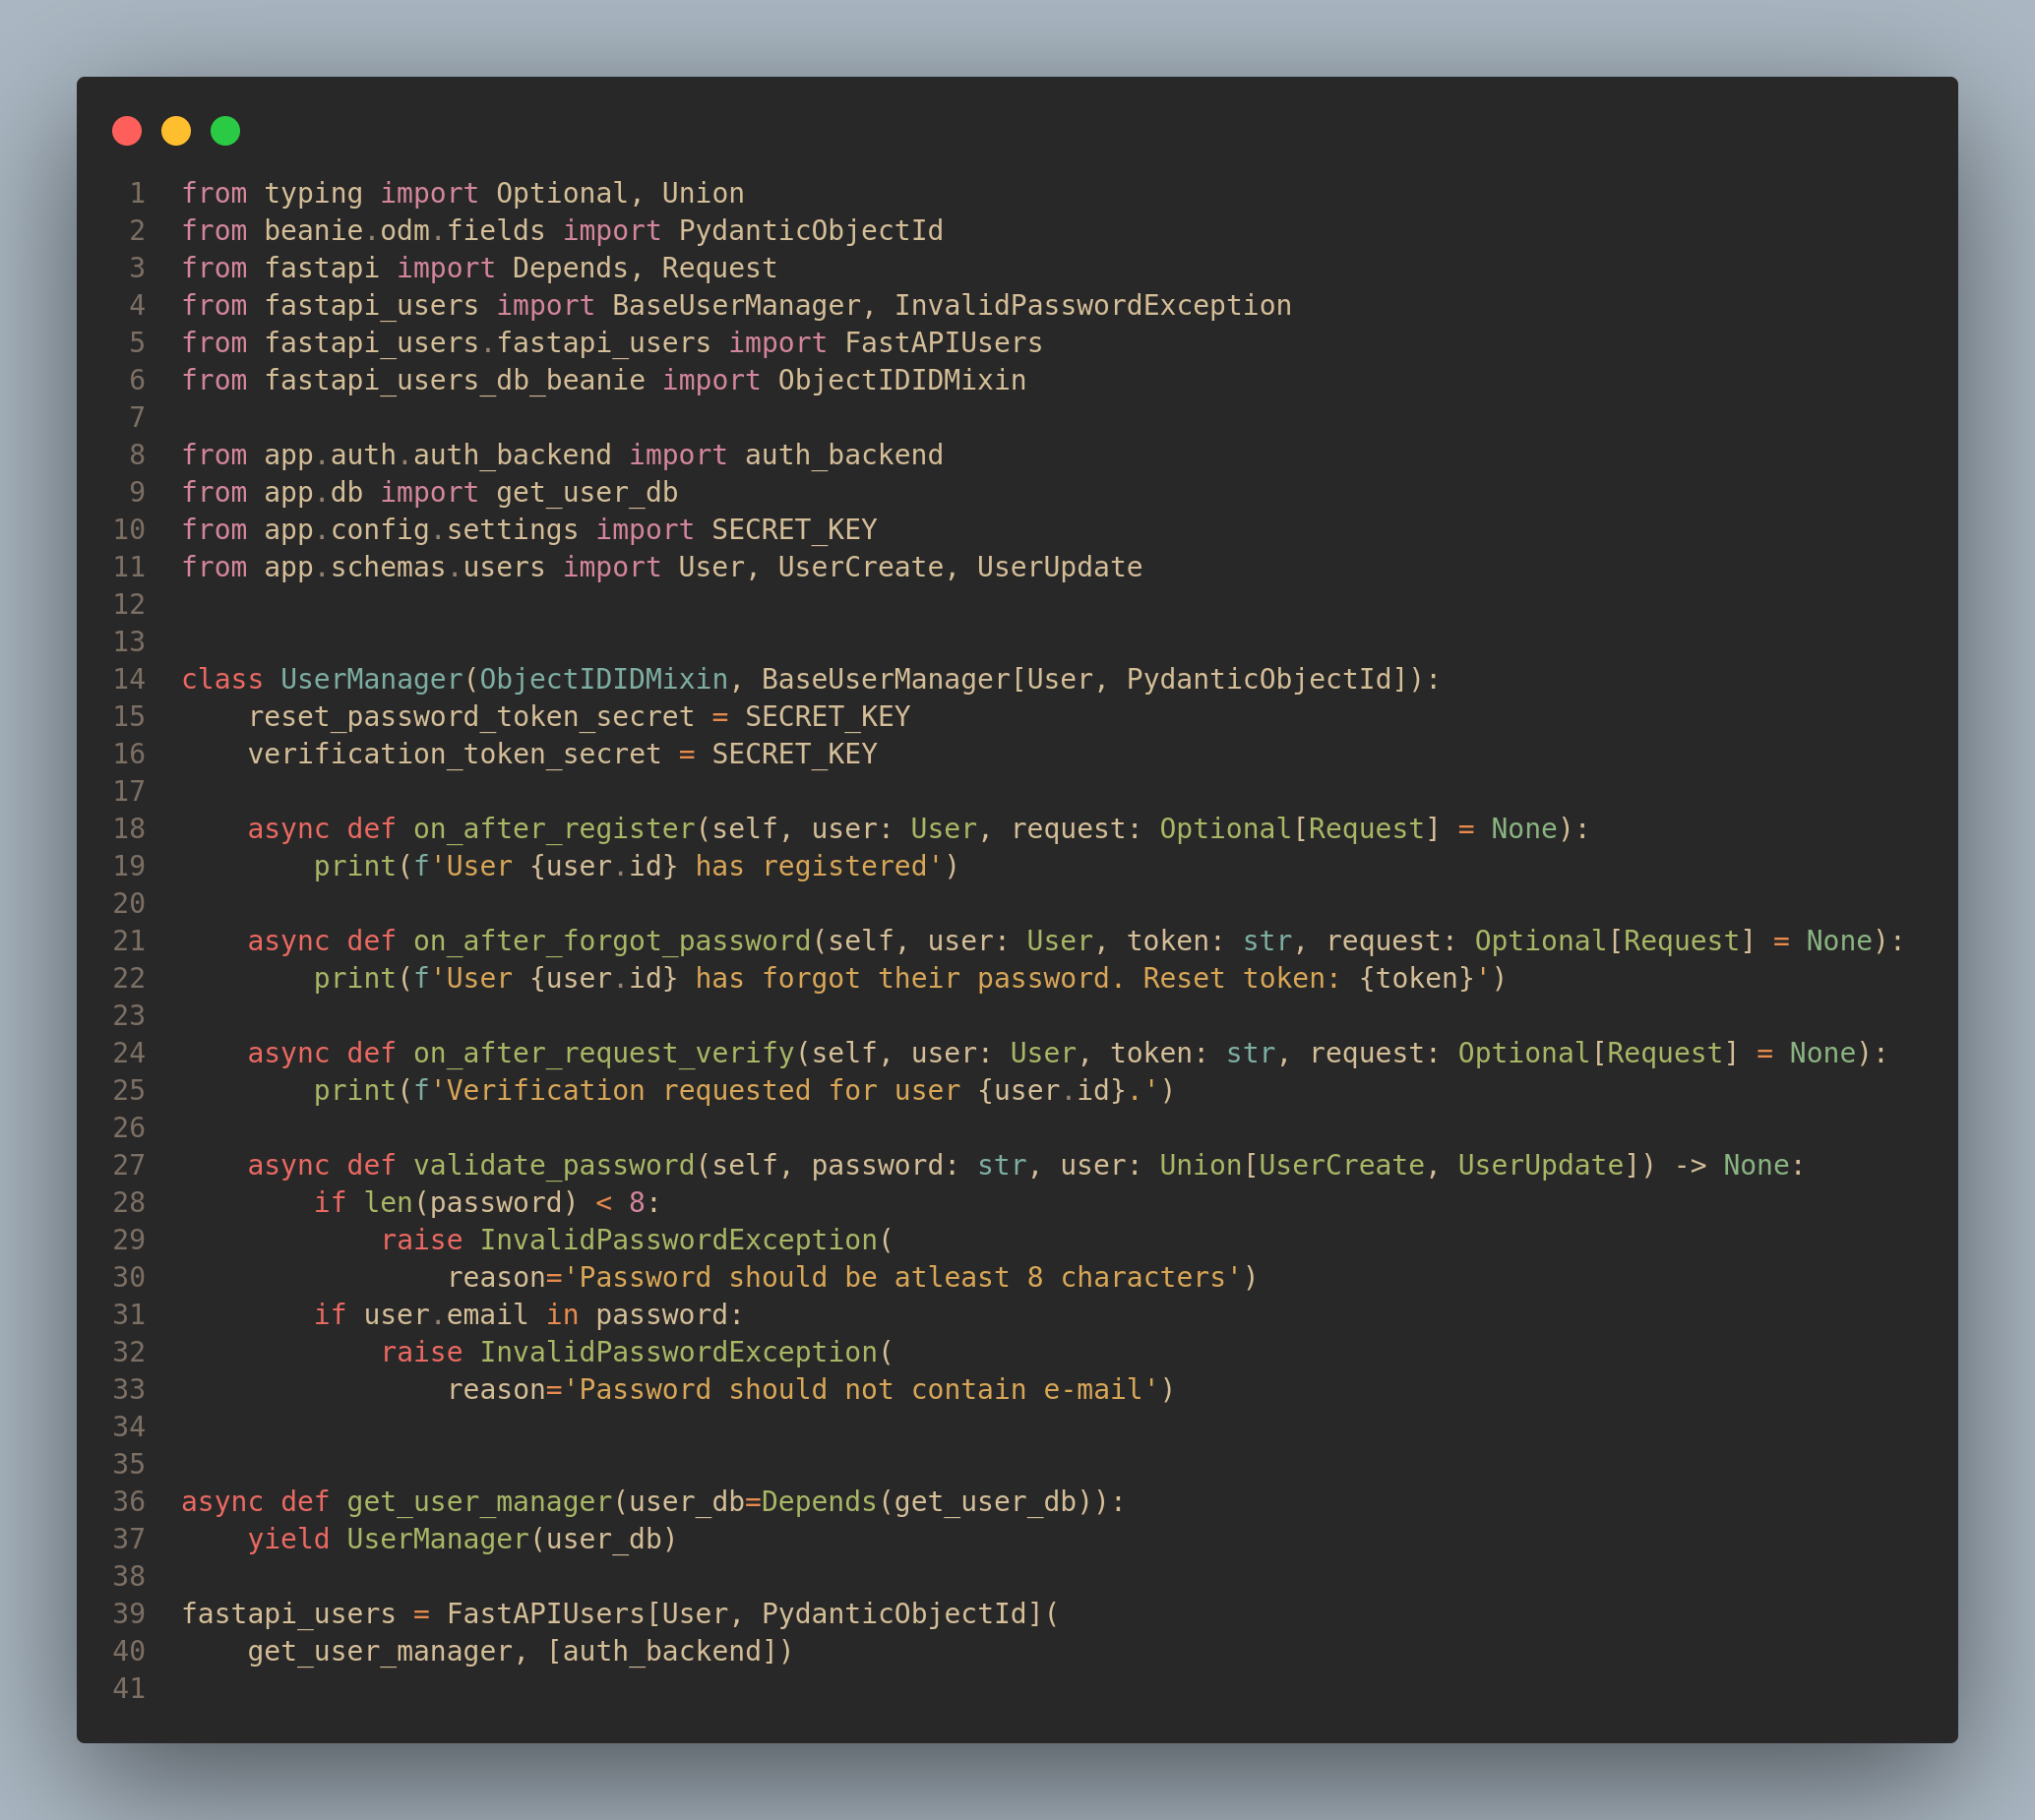
\includegraphics[width=\textwidth]{chapter-5/api-login-manager}
    \caption{API login manager with fastapi-users}
    \label{code:api-login-manager}
\end{figure}

\begin{figure}
    \centering
    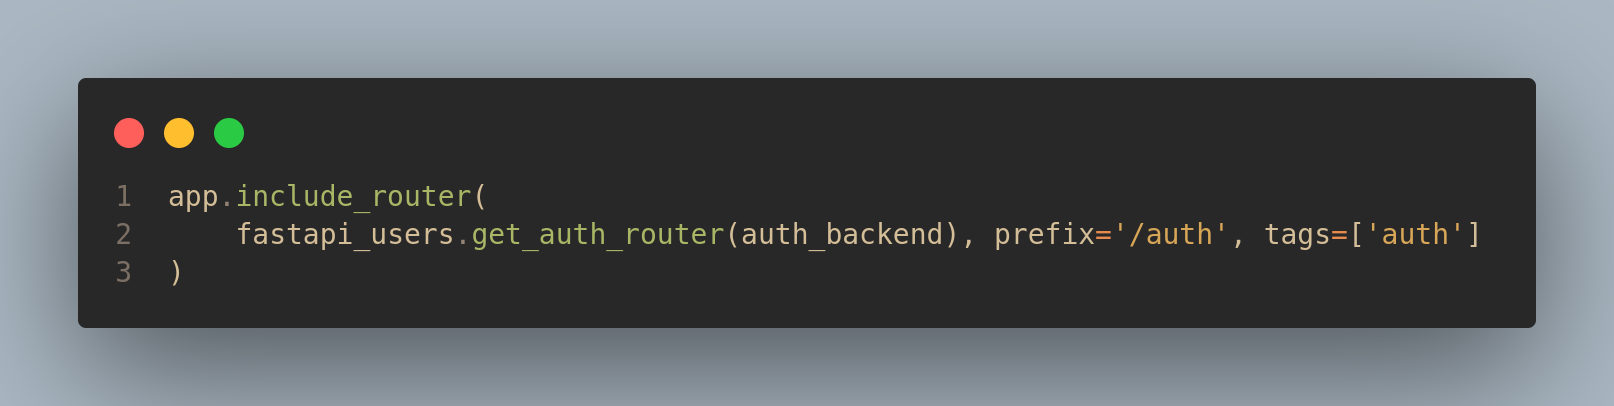
\includegraphics[width=\textwidth]{chapter-5/api-include-auth-router}
    \caption{API auth router with fastapi-users}
    \label{code:api-auth-router}
\end{figure}

\paragraph{Stateless Authentication}
The security control \emph{4.3} states \say{If stateless token-based authentication is used, the server provides a token that has been signed using a secure algorithm}. The fastapi-users library allows connecting to a Redis database to securely store user tokens that are created upon user authentication and destroyed when logging out. This is handled by the library itself. 

\paragraph{Authorization Model}
The created token also puts in place a mechanism that allows or denies the user access to an endpoint. As a result security control \emph{4.12} from table \ref{tab:auth-and-session-summary-requirements} can also be marked as done and implemented. 

\paragraph{Session Timeout}
Lastly, the token lifetime is set. That way sessions are invalidated at the remote endpoint after a predefined period of inactivity as required by security control \emph{4.7}.

\section{Client-side Implementation}
React Native together with the Expo SDK provides means to implement security. In this section the security implementation is presented for the client side. As seen in table \ref{tab:sec-controls-client} not all security controls have been implemented unlike the API security controls.

\begin{table}
    \centering
    \caption{Implemented security controls on client side}
    \label{tab:sec-controls-client}
    \begin{tabulary}{1.0\textwidth}{|L|L|l|}
        \hline
        \textbf{ID} & \textbf{Security Control} & \textbf{Done} \\
        \hline
        \textbf{2.1} & System credential storage facilities need to be used to store sensitive data, such as PII, user credentials or cryptographic keys & Yes \\
        \hline
        \textbf{2.2} & No sensitive data should be stored outside of the app container or system credential storage facilities & No \\
        \hline
        \textbf{2.3} & No sensitive data is written to application logs & Yes \\
        \hline
        \textbf{2.5} & The keyboard cache is disabled on text inputs that process sensitive data & No \\
        \hline
        \textbf{2.6} & No sensitive data is exposed via IPC mechanisms & No \\
        \hline
        \textbf{2.7} & No sensitive data, such as passwords or pins, is exposed through the user interface & No \\
        \hline
    \end{tabulary}
\end{table}

\subsection{Authentication and Session Management}
The client-side primarily concerns about the user interface and the user experience. However, user authentication and user access control has to be implemented as well. For example, during the requirements gathering phase it has already been established that tokens that are generated by the remote endpoint need to be stored on the client side in order to provide a better user experience and permitting access to certain content and functions of CheFeed.

\paragraph{Local Storage for Sensitive Data}
The only sensitive data CheFeeds requires storing locally is the user authorization token. Besides the benefit of the user not needing to log in every time the user wants to use the app, it also provides the user authorization to certain functions within CheFeed such posting recipes. To achieve secure local storage CheFeeds implements the \emph{SecureStorage} API provided by Expo. The API allows data encryption and decryption using the local storage API from both Android and iOS devices. The implementation is seen in figure \ref{code:secure-storage-client}. In figure \ref{code:client-authenticate} is shown how the \verb|storeAccessToken()| function is used in the \verb|authenticateUser()| function on line 16. Here it is ensured that whenever the user is authenticated, the token received by the remote endpoint is stored securely.

\begin{figure}
    \centering
    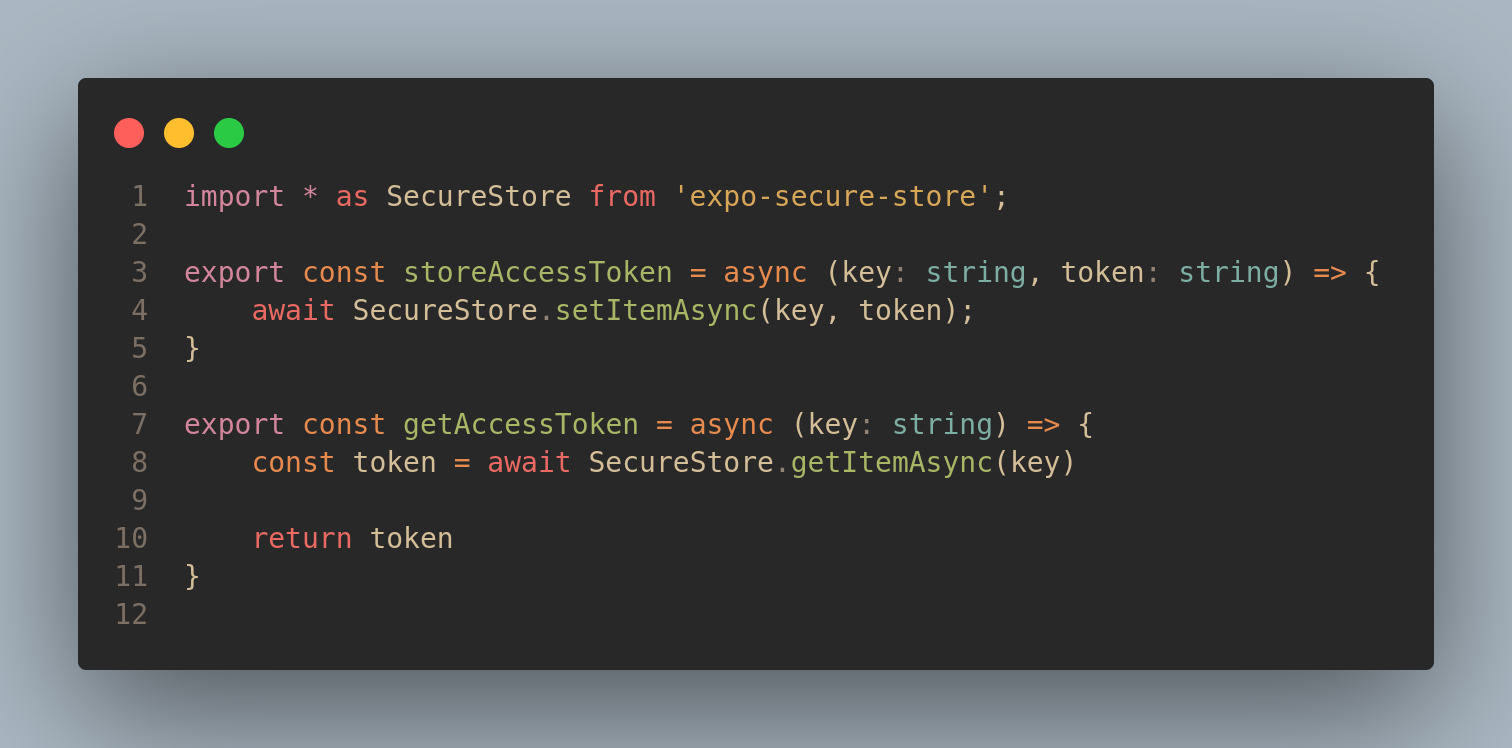
\includegraphics[width=\textwidth]{chapter-5/securestorage}
    \caption{Client secure storage}
    \label{code:secure-storage-client}
\end{figure}

\begin{figure}
    \centering
    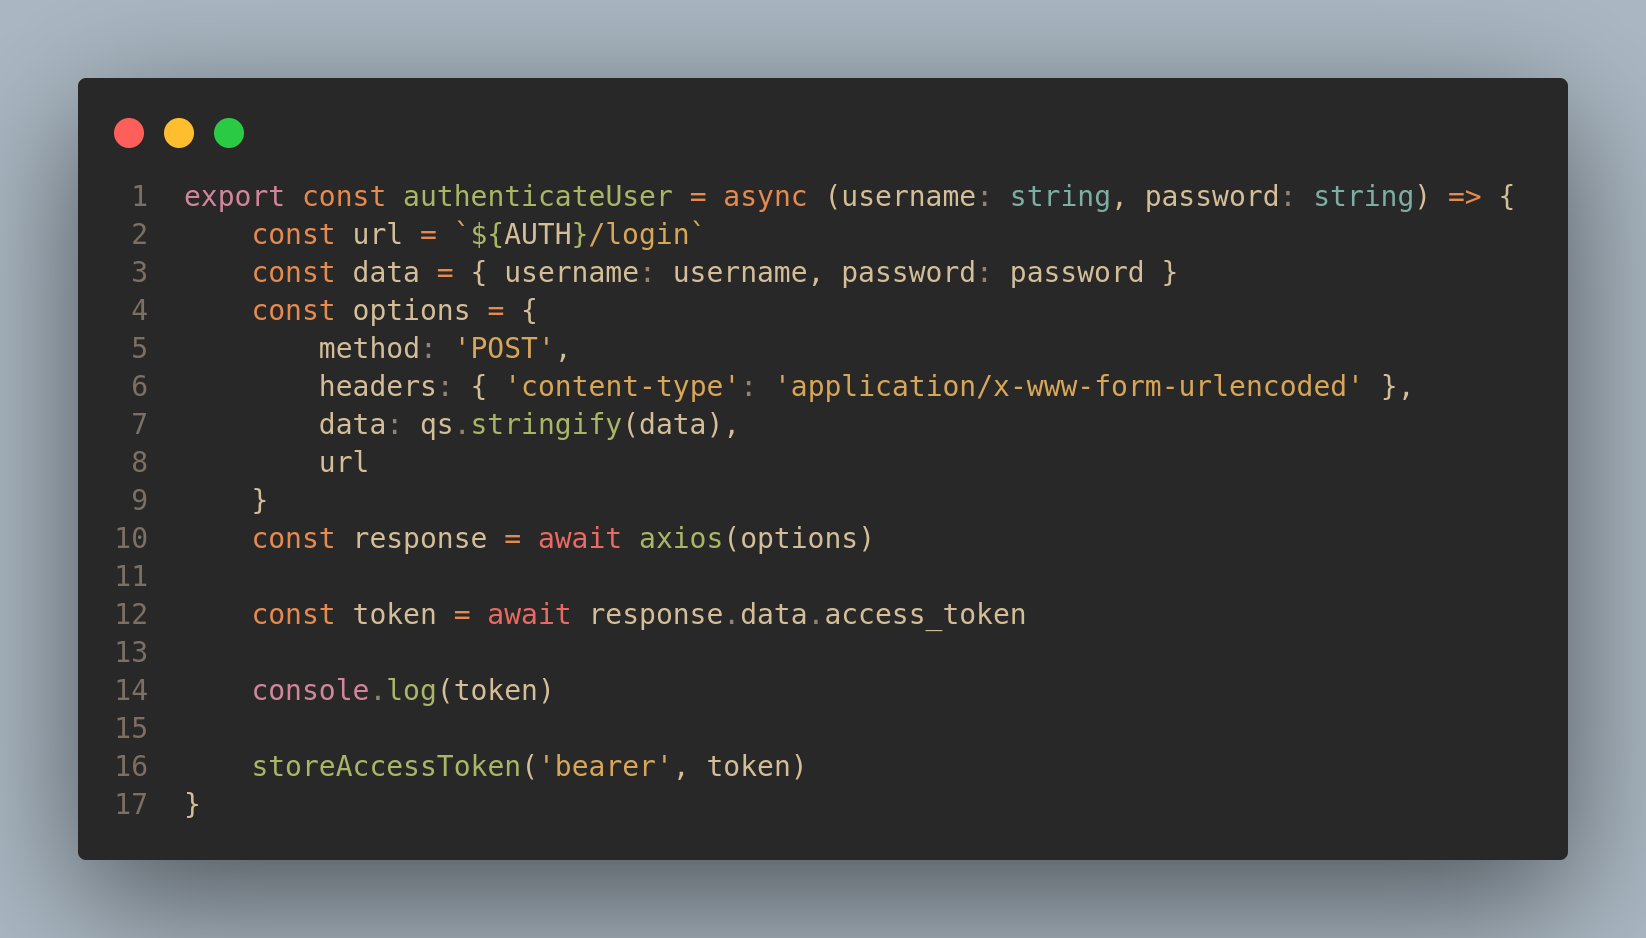
\includegraphics[width=\textwidth]{chapter-5/authenticate}
    \caption{Client authentication}
    \label{code:client-authenticate}
\end{figure}
